\documentclass[11pt]{article}
\usepackage[margin=1in]{geometry} 
\usepackage{amsmath,amsthm,amssymb,amsfonts}

\usepackage{mathpazo}
\usepackage{euler}
\usepackage{xcolor}
\usepackage{tikz}
\usepackage{tikz-cd}
\usetikzlibrary{arrows}
\usetikzlibrary{matrix}
\usepackage{fancyhdr}
\pagestyle{fancy}

\newcommand{\N}{\mathbb{N}}
\newcommand{\Z}{\mathbb{Z}}
\newcommand{\Q}{\mathbb{Q}}
\newcommand{\R}{\mathbb{R}}
\newcommand{\C}{\mathbb{C}}
\newcommand{\Ss}{\mathbb{S}}
\newcommand{\M}[2]{\mathsf{M}_{#1}#2}
\newcommand{\im}{\operatorname{im}}
\newcommand{\eps}{\varepsilon}
\newcommand{\dpart}[2]{\frac{\partial#1}{\partial#2}}
\newcommand{\nat}[1]{[\![#1]\!]}
\newcommand{\natzero}[1]{\nat{#1}_0}
\newcommand{\adj}[1]{\operatorname{adj}(#1)}
\newcommand{\ip}[2]{\langle #1 , #2 \rangle}
\newcommand{\paint}[2]{\color{#1}{#2}}
\newcommand{\ol}{\overline}
\newcommand{\hook}[3]{\frac{\partial}{\partial x_{#1}}\Big\rvert_{#2}^{#3}}
\usepackage{rotating}
\newcommand*{\isoarrow}[1]{\arrow[#1,"\rotatebox{90}{\LARGE{\(\sim\)}}"
]}
\definecolor{red}{RGB}{244, 66, 66}

\renewcommand*{\proofname}{\paint{red}{Demostraci\'on}}
\newenvironment{theorem}[2][Teorema]{\begin{trivlist}
\item[\hskip \labelsep \paint{red}{{\bfseries #1}}\hskip \labelsep {\bfseries #2.}]}{\end{trivlist}}
\newenvironment{lemma}[2][Lema]{\begin{trivlist}
\item[\hskip \labelsep \paint{red}{{\bfseries #1}}\hskip \labelsep {\bfseries #2.}]}{\end{trivlist}}
\newenvironment{exercise}[2][Ejercicio]{\begin{trivlist}
\item[\hskip \labelsep \paint{red}{{\bfseries #1}}\hskip \labelsep {\bfseries #2.}]}{\end{trivlist}}
\newenvironment{obs}[2][Observaci\'on]{\begin{trivlist}
\item[\hskip \labelsep \paint{red}{{\bfseries #1.}}]}{\end{trivlist}}
\newenvironment{reflection}[2][Resoluci\']{\begin{trivlist}
\item[\hskip \labelsep {\bfseries #1}\hskip \labelsep {\bfseries #2.}]}{\end{trivlist}}
\newenvironment{proposition}[2][Proposici\'on]{\begin{trivlist}
\item[\hskip \labelsep \paint{red}{{\bfseries #1.}}]}{\end{trivlist}}
\newenvironment{corollary}[2][Corolario]{\begin{trivlist}
\item[\hskip \labelsep {\bfseries #1}\hskip \labelsep {\bfseries #2.}]}{\end{trivlist}}

%-----------------------

\title{
\LARGE{\paint{red}{Geometr\'ia Diferencial}}
\\
\vspace{0.5pt}
\small{\paint{red}{Ejercicios para Entregar - Pr\'actica 2}}
}
\author{\paint{red}{Guido Arnone}}
\date{}
\lhead{Guido Arnone}
\rhead{Pr\'actica 2}

\begin{document}

\maketitle

\begin{center}
\paint{red}{\large{Sobre los Ejercicios}}
\end{center}
\begin{center}
Adem\'as del ejercicio $\paint{red}{(9)}$, elej\'i resolver los ejercicios $\paint{red}{(4)}$ y $\paint{red}{(12)}$.
\end{center}
\begin{center}
$\paint{red}{
\rule{400pt}{0.5pt}
}$
\vspace{35pt}
\end{center}

\begin{exercise}{4} Sea $f:M\to N$ una funci\'on diferenciable entre variedades de la misma dimensi\'on y supongamos que su dominio es compacto.
\begin{itemize}
\item[(a)] Para cada $q\in N$ que es un valor regular de $f$ el conjunto $f^{-1}(q)$ es finito.
\item[(b)] Sea $R$ el conjunto de los valores regulares de~$f$. El conjunto $R$ es un abierto de $N$ y la funci\'on 
  \[
  q\in R\mapsto\#f^{-1}(q)\in\N_0
  \]
es localmente constante. ¿Es necesariamente constante?
\end{itemize}
\end{exercise}
\begin{proof} Veamos primero el inciso $\paint{red}{(a)}$. Fijemos $q \in N$ un valor regular. Como $f$ es diferenciable en particular es continua y entonces el conjunto $E_q := f^{-1}(q)$ es un cerrado de $M$, al ser la preimagen del cerrado $\{q\} \subset N$. Como $E_q$ es un cerrado y $M$ es compacta, el primero resulta compacto. Por lo tanto, para probar que $E_q$ es finito alcanza con mostrar que es discreto con la topolog\'ia subespacio de $M$. Concretamente, basta ver que si $p \in E_q$ entonces existe $U \subset M$ abierto con $U \cap E_q = \{p\}$. Si $p \in E_q$, como $q$ es un valor regular $d_pf :T_pM \to T_qN$ es sobreyectiva. Por otro lado, por hip\'otesis sabemos que $\dim T_pM = \dim M = \dim N = \dim T_qN$. Como $d_pf$ es una funci\'on lineal sobreyectiva entre espacios vectoriales de la misma dimensi\'on, es un isomorfismo. El teorema de la funci\'on inversa nos asegura entonces que existen abiertos $U \ni p$ y $V \ni q$ de $M$ y $N$ respectivamente tales que la (co) restricci\'on $f|_U^V : U \to V$ de $f$ es un difeomorfismo. En particular $f|_U^V$ es inyectiva y entonces la preimagen de un punto contiene a lo sumo un elemento. Se tiene entonces que
\begin{align*}
U \cap f^{-1}(q) \stackrel{(q \in V)}{=} ({f|^V_U)}^{-1}(q) \stackrel{(p \in U)}{=} \{p\},
\end{align*}
lo que concluye la prueba de $\paint{red}{(a)}$. 

Ahora veamos $\paint{red}{(b)}$. Fijemos $q \in R$. Si $q \not \in f(M)$, entonces $\#f^{-1}(q) = 0$. Como $M$ es compacta y $N$ es Hausdorff pues es una variedad, $f$ es cerrada. Entonces $f(M)$ es cerrado y por lo tanto, $f(M)^c$ es un abierto que contiene a $q$. All\'i (vacuamente) todo punto es regular y tiene preimagen de tamaño cero: basta probar la afirmaci\'on para $q \in R \cap f(M)$. Sea $f^{-1}(q) = \{p_1, \dots, p_k\}$. Aplicando el argumento que usamos en $\paint{red}{(a)}$ a cada punto $p_i$, obtenemos abiertos $(A_i)_{i=1}^k$ de $M$ y $(B_i)_{i=1}^k$ de $N$ tales que las restricciones $f|_{A_i}^{B_i} : A_i \to B_i$ de $f$ son difeomorfismos con $p_i \in A_i$ y $q \in B_i$ para todo $i \in \nat{k}$. M\'as a\'un podemos garantizar\footnote{Como $M$ es Hausdorff, existen entornos abiertos $U_i \ni p_i$ para cada $i \in \nat{k}$ disjuntos dos a dos. Luego las (co) restricciones $f : A_i \cap U_i \to f(A_i \cap U_i)$ siguen siendo difeomorfismos y los abiertos $(A_i \cap U_i)_{i=1}^k$ son disjuntos dos a dos. Por lo tanto, podemos suponer directamente que los abiertos lo eran.} que $A_i \cap A_j = \emptyset$ si $i \neq j$. Definimos ahora $B = \cap_{i \in \nat{k}}B_i$ y $U_i := (f|_{A_i}^{B_i})^{-1}(B)$ para cada $i \in \nat{k}$. Las (co)restricciones

\begin{align*}
f|_{U_i}^{B} : U_i \to B
\end{align*}

con $1 \leq i \leq k$ resultan entonces difeomorfismos.

Definimos\footnote{Dado $q' \in B$, nos gustar\'ia afirmar que su preimagen cae enteramente en la uni\'on de los abiertos $U_i$ pues esto implicar\'ia que es un valor regular. Esto no es necesariamente cierto, al menos a simple vista. Intuitivamente, forzamos esta situaci\'on quitandole a $B$ los puntos de $f(C)$, y luego corestringiendo apropiadamente conseguimos nuevos abiertos en $M$ y $N$ que cumplen con lo que buscamos.} ahora $C = (\cap_{i \in \nat{k}} U_i)^c$. Como $f$ es cerrada, $f(C)$ es cerrado. Ahora, una vez m\'as: definimos los abiertos $V := B \setminus f(C)$ y $O_i := (f|_{U_i}^B)^{-1}(V) \stackrel{(V \subset B)}{=} U_i \cap f^{-1}(V)$, de forma que cada restricci\'on $f|_{O_i}^V: O_i \to V$ sigue siendo un difeomorfismo. Afirmamos ahora que $f^{-1}(V) = \bigcup_{i \in \nat{k}}O_i$. Por definici\'on ya sabemos que $f^{-1}(V) \supseteq \bigcup_{i \in \nat{k}}O_i$. Rec\'iprocamente si $x \in f^{-1}(V)$ entonces $f(x) \not \in f(C)$ y por lo tanto $x \not \in C $. Entonces $x \in C^c = \bigcup_{i \in \nat{k}}U_i$. Como partimos de que $x \in f^{-1}(V)$, efectivamente obtenemos que

\begin{align*}
x \in f^{-1}(V) \cap \bigcup_{i \in \nat{k}}U_i = \bigcup_{i \in \nat{k}}(f^{-1}(V) \cap U_i) = \bigcup_{i \in \nat{k}}O_i.
\end{align*} 

Veamos que esto implica ambas afirmaciones de $\paint{red}{(b)}$. Por un lado, si $p \in f^{-1}(V)$ entonces $p \in O_i$ para alg\'un $i \in \nat{k}$ y como $f|_{O_i}^V$ es un difeomorfismo entonces via los isomorfismos $T_pO_i \simeq T_pM$ y $T_{q'}V \simeq T_{q'}N$, tenemos que $d_pf$ es un isomorfismo:

\begin{center}
\begin{tikzcd}
T_pM \arrow{r}{d_pf} \isoarrow{d} & T_{q'}N \isoarrow{d}\\ 
T_pO_i \arrow{r}{d_pf|_{O_i}^V} & T_{q'}V
\end{tikzcd}
\end{center}
En particular $d_pf$ resulta sobreyectivo. Como $p \in f^{-1}(q')$ era arbitario, vemos que para cada punto en la preimagen de $q'$ el diferencial all\'i es sobreyectivo: esto quiere decir que $q'$ es un punto regular, y como $q' \in V$ era arbitrario, es $V \subset R$. Esto prueba que $R$ es abierto: partimos de un punto $q \in R$ y obtuvimos un entorno abierto $V \ni q$ contenido en $R$. Adem\'as, para cada $q' \in V$ tenemos que $f^{-1}(q') \subset f^{-1}(V) \subset \bigcup_{i \in \nat{k}}O_i$ as\'i que

\begin{align*}
f^{-1}(q') = f^{-1}(q') \cap \bigcup_{i \in \nat{k}}O_i = \bigcup_{i \in \nat{k}}(O_i \cap f^{-1}(q')) = \bigcup_{i \in \nat{k}}f|_{O_i}^V(q').
\end{align*}

Como los conjuntos $(O_i)_{i \in \nat{k}}$ son disjuntos dos a dos pues $O_i \subset A_i$ para cada $i$, \'asi que de la anterior igualdad es $\#f^{-1}(q') = \sum_{i=1}^k\#({f|_{O_i}^V}^{-1}(q'))$. Cada restricci\'on $f|_{O_i}^V$ es biyectiva (pues es un difeomorfismo), de modo que la preimagen de $q'$ en cada caso tiene exactamente un punto:

\begin{align*}
f^{-1}(q') = \sum_{i=1}^k\#(f|_{O_i}^V(q')) = \sum_{i=1}^{k}1 = k = \#f^{-1}(q).
\end{align*}

Como esto es cierto para cualquier $q' \in V$, la aplicaci\'on $q \in R \mapsto \#f^{-1}(q) \in \N_0$ es localmente constante. 

Por \'ultimo, observemos que en general \textbf{no es cierto que la aplicaci\'on sea constante}. Veamos el siguiente contraejemplo: tomamos $M = N = S_1 \sqcup S_2$ con $S_1 = S_2 = \Ss^1$ que es una variedad compacta, con las inclusiones $j_i : \Ss^1 = S_i \hookrightarrow S_1 \sqcup S_2$ diferenciables\footnote{Tomamos la topolog\'ia coproducto y las siguientes cartas: para cada carta $(U,\varphi)$ en el atlas maximal de $\Ss^1$ tenemos dos cartas $(U_i,\varphi_i)$ con $U_i = U$ visto en $S_i$ y $\varphi_i = \varphi$ bajo la misma identificaci\'on. Por lo tanto, si $p \in \Ss^1$, tomamos $(U,\varphi)$ una carta de $\Ss^1$ con $U \ni p$ y $(U_i,\varphi_i)$ en $S_1 \sqcup S_2$. Entonces $\varphi_ij_i\varphi^{-1} = \varphi^{-1}\varphi = id_{\varphi(U)}$. Esto dice que las inclusiones $j_1,j_2$ resultan diferenciables.}. Si $f_1,f_2 : \Ss^1 \to \Ss^1$ son diferenciables, entonces $f_1 \sqcup f_2 : S_1 \sqcup S_2 \to S_1 \sqcup S_2$ lo es: basta probar diferenciabilidad restringiendo a los abiertos $S_1$ y $S_2$. Esto es como ver que la precomposici\'on por las inclusi\'ones es diferenciable, lo que es cierto pues \'esta se factoriza por las aplicaciones $j_i$ y $f_i$, todas diferenciables:

\begin{center}
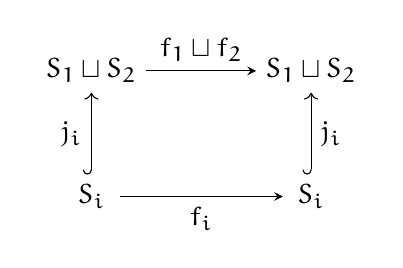
\begin{tikzpicture}
  \matrix (m) [matrix of math nodes,row sep=3em,column sep=4em,minimum width=2em]
  {
     S_1 \sqcup S_2 & S_1 \sqcup S_2\\
     S_i  & S_i\\};
  \path[-stealth]
    (m-1-1) edge node [above] {$f_1 \sqcup f_2$} (m-1-2)
    (m-2-1) edge [right hook->] node [left] {$j_i$}(m-1-1)
    (m-2-1) edge node [below] {$f_i$} (m-2-2)
    (m-2-2) edge [right hook->] node [right] {$j_i$}(m-1-2);
\end{tikzpicture}
\end{center}
Del diagrama anterior y usando que las inclusiones de abiertos inducen isomorfismos en los tangentes, tenemos para cada $p \in S_i$ que
\begin{center}
\begin{tikzcd}
T_pS_i \arrow{r}{d_pf_i}  \isoarrow{d} & T_{f_i(p)}S_i \isoarrow{d}\\ 
T_p(S_1 \sqcup S_2) \arrow{r}{d_pf_1 \sqcup f_2}& T_{f_i(q)}(S_1 \sqcup S_2)
\end{tikzcd}
\end{center}
conmuta. Como $f_1,f_2$ y $f_1 \sqcup f_2$ son funciones entre variedades de igual dimensi\'on, sus diferenciales son sobreyectivos si y s\'olo si son isomorfismos. En particular, si $q \in S_i$ es un valor regular para $f_i$ es tambi\'en un valor regular para $f_1 \sqcup f_2$.

Ahora, pasemos a una funci\'on concreta: tomamos $g : z \in \Ss^1 \mapsto z^2 \in \Ss^1$, pensando a $\Ss^1 \subset \C$, y consideramos $id \sqcup g$. Por la observaci\'on anterior, todo punto $p$ de $S_1$ es regular, y su preimagen es exactamente $\{p\} \subset S_1$. Por otro lado, si $p \in S_2$ es $\#(id \sqcup g )^{-1}(p) = \#g^{-1}(p) = 2$. Por lo tanto, resta probar que existe alg\'un valor regular $p \in \Ss^1$ de $g$ para concluir que la funci\'on $q \in R \mapsto (id \sqcup g)^{-1}(p)$ en este caso no es constante. M\'as a\'un, como los tangentes en este caso son $1$-dimensionales, basta ver que existe $p \in \Ss^1$ tal que $d_pg$ es no nulo, pues en tal caso ser\'a sobreyectivo\footnote{Como $\Ss^1$ es conexa y $g$ no es constante, el ejercicio $\paint{red}{(12)}$ que resolvemos m\'as adelante garantiza que debe existir cierto $p \in \Ss^1$ para el cual es $d_pg \neq 0$. De todas formas, optamos por una resoluci\'on elemental.}. Veamos que $d_{(1,0)}g$ es no nulo. Para esto, consideramos la carta

\begin{align*}
\varphi : (x,y) \in \{(x,y) \in \Ss^1 : x > 0\} \mapsto y \in (-1,1)
\end{align*}

alrededor de $(0,1)$. Como $g(1,0) = (1,0)$, luego $\frac{d}{dt}\Big|_{(1,0)}^\varphi$ es una derivaci\'on en $(1,0)$ y entonces basta con ver que

\begin{align*}
d_{(0,1)}g\left(\frac{d}{dt}\Big|_{(1,0)}^\varphi\right)(\varphi) = \frac{d}{dt}\Big|_{(1,0)}^\varphi(\varphi g) = \frac{d(\varphi g\varphi^{-1})}{dt}\Big|_0
\end{align*}

es distinto de cero para concluir que $d_{(1,0)}g \neq 0$. Como $g(x,y) = (x^2 -y^2,2xy)$, es

\begin{align*}
\varphi g\varphi^{-1}(y) = \varphi g(\sqrt{1-y^2},y) = \varphi(1-y^2-y^2,2\sqrt{1-y^2}y) = 2y\sqrt{1-y^2}
\end{align*}

y entonces $\frac{d(\varphi g\varphi^{-1})}{dt} = \frac{2-4y^2}{\sqrt{1-y^2}}$. Por lo tanto,

\begin{align*}
d_{(0,1)}g\left(\frac{d}{dt}\Big|_{(1,0)}^\varphi\right)(\varphi) =  \frac{2-4y^2}{\sqrt{1-y^2}}\Bigg|_0 = 2 \neq 0.
\end{align*}

Esto termina de mostrar que si bien la aplicaci\'on del ejercicio es localmente constante, no necesariamente resulta constante. 

\end{proof}

\begin{exercise}{9} Sea $M$ una variedad diferenciable de dimensi\'on $n$ y $\mathcal{A}$ su atlas maximal. Sea $TM=\bigsqcup_{p\in M}T_pM$ y sea $\pi :TM\to M$ la funci\'on tal
que $\pi (v)=p$ si $v\in T_pM$. Para cada $(U,x)\in \mathcal{A}$, sea
$TU=\bigsqcup_{p\in U}T_pM\subset TM$ y $\ol{x}:TU\to
x(U)\times \R^{n}$ la funci\'on tal que
  \[
  \ol{x}(v)=(x(\pi (v)),v(x^{1}),\dots ,v(x^{n}))
  \]
cada vez que $v\in TU$. Probar que:
\begin{itemize}
\item[(a)] La funci\'on $\ol{x}:TU\to x(U)\times \R^{n}$ es una biyecci\'on
con inversa
  \[
  \ol{x}^{-1}(a,b^{1},\dots,b^{n})
        = \sum_{i=1}^{n}b^{i}\frac{\partial}{\partial x^{i}}\Big|_{x^{-1}(a)}
  \]
para cada $a\in x(U).$

\item[(b)] Si $(U,x)$,~$(V,y)\in \mathcal{A}$ y $U\cap V\neq\emptyset$, entonces $\ol{x}(TU\cap
TV) = x(U\cap V)\times\R^{n}$ es un abierto de $\R^{2n}$ y 
la biyecci\'on $\ol{x}\circ \ol{y }^{-1}:y(U\cap V)\times\R^{n}\to x(U\cap V)\times 
\R^{n}$ es un difeomorfismo.

\item[(c)] El conjunto $TM$ admite una estructura diferenciable que lo transforma en
una variedad diferenciable de dimensi\'on $2n$, con atlas
  \[
  \ol{\mathcal{A}}=\{(TU,\ol{x}):(U,x)\in\mathcal{A}\}.
  \]

\item[(d)] Con respecto a esta estructura diferenciable, la proyecci\'on $\pi :TM\to M$ es diferenciable.
\end{itemize}
\end{exercise}
\begin{proof} Hacemos cada inciso por separado,
\begin{itemize}
\item[(a)] Sean $(a,b) = (a, b^1, \dots, b^n) \in x(U) \times \R^n$ y $h(a,b) := \sum_{i=1}^nb^i \frac{\partial}{\partial x_i}|_{x^{-1}(a)}$. Como $h(a,b)$ es una combinaci\'on lineal de derivaciones en $x^{-1}(a)$, resulta una derivaci\'on en $x^{-1}(a)$. Por lo tanto, $h(a,b) \in T_{x^{-1}(a)}M$ y entonces $x\pi(h(a,b)) = xx^{-1}(a) = a$. Adem\'as, si $\pi_j : \R^n \to \R$ es la proyecci\'on en la $j$-\'esima coordenada, para cada $j \in \nat{n}$ es $x^j = \pi_jx$ y entonces
\begin{align*}
h(a,b)(x^j) &= \left(\sum_{i=1}^nb^i \hook{i}{x^{-1}(a)}{} \right)(x^j) = \sum_{i=1}^nb^i \hook{i}{x^{-1}(a)}{}(x^j) = \sum_{i=1}^nb^i \frac{\partial (x^jx^{-1})}{\partial x_i}\Big|_a \\
& = \sum_{i=1}^nb^i \frac{\partial \pi_j}{\partial x_i}\Big|_a =  \sum_{i=1}^nb^i \delta_{ij} = b^j.
\end{align*}
Concluimos as\'i que $\ol{x}(h(a,b)) = (a,b) \in x(U) \times \R^n$. Rec\'iprocamente si $v \in M_p$ con $p \in U$, luego
\begin{align*}
h(\ol{x}(v)) & = h(x\pi(v),v(x^1),\dots,v(x^n)) = \sum_{i=1}^nv(x^i)\hook{i}{x^{-1}(x\pi(v))}{} = \\
& = \sum_{i=1}^nv(x^i)\hook{i}{p}{}.
\end{align*}
Esto \'ultimo coincide justamente la expresi\'on de $v$ en la base $\big\{\hook{i}{p}{}\big\}_{i=1}^n$, lo que termina de probar que $h = \ol{x}^{\ -1}$.
\item[(b)] En primer lugar, notemos que como $U \cap V$ es abierto y $x$ homeomorfismo, $x(U\cap V)$ es abierto y as\'i $x(U \cap V) \times \R^n$ es abierto en $\R^{2n}$. Tenemos tambi\'en que $TU \cap TV = T(U \cap V)$ y usando $\paint{red}{(a)}$, es $\ol{x|_{U \cap V}} = \ol{x}|_{T(U \cap V)}$ por lo que $\ol{x|_{U \cap V}}$ resulta sobreyectiva (ya que $x|_{U \cap V}$ es otra carta de $M$). Luego $\paint{red}{(b)}$ nos dice que en efecto $\ol{x}(TU \cap TV) = x(U \cap V) \times \R^n$. 

Veamos ahora que $\ol{x}\ol{y}^{-1}$ es un difeomorfismo. Como $\ol{x}$ e $\ol{y}$ son biyectivas, basta ver que las composiciones $\ol{x}\ol{y}^{-1}$ y $\ol{y}\ol{x}^{-1}$ son diferenciables. Por simetr\'ia (ya que podemos intercambiar los roles de $x$ e $y$) basta probar un caso: lo hacemos para $\ol{x}\ol{y}^{-1}$. Por un c\'alculo directo, si $(a,b) \in y(U\cap V) \times \R^n$ y $\pi_j : \R^n \to \R$ es la proyecci\'on en la $j$-\'esima coordenada, para cada $j \in \nat{n}$ es $x^jy^{-1} = \pi_jxy^{-1} = (xy^{-1})^j$. Por lo tanto,
\begin{align*}
\ol{y}^{-1}(a,b)(x^j) &= \sum_{i=1}^n b^i \frac{\partial}{\partial y_i}\Big|_{y^{-1}(a)}(x^j) = \sum_{i=1}^nb^i \frac{\partial x^jy^{-1}}{\partial x_i}\Big|_a \\ & = \sum_{i=1}^nb^i \frac{\partial (xy^{-1})^j}{\partial x_i}\Big|_a = [\mathbb{J}(xy^{-1})_a \cdot b]_j
\end{align*}
con $\mathbb{J}(xy^{-1})_a$ la matriz jacobiana de $xy^{-1}:y(U \cap V) \subset \R^n \to x(U \cap V) \subset \R^n$ en el punto $a \in y(U \cap V)$. Por $\paint{red}{(a)}$ sabemos que $\pi \ol{y}^{-1}(a,b) = y^{-1}(a)$, as\'i que
\begin{align*}
x\ol{y}^{-1}(a,b) & = (x\pi(\ol{y}^{-1}(a,b)),\ol{y}^{-1}(a,b)(x^1), \dots, \ol{y}^{-1}(a,b)(x^n)) \\ 
& = (xy^{-1}(a),[\mathbb{J}(xy^{-1})_a \cdot b]_1, \dots, [\mathbb{J}(xy^{-1})_a \cdot b]_n)\\
& = (xy^{-1}(a),\mathbb{J}(xy^{-1})_a \cdot b).
\end{align*}
Como $M$ es variedad diferenciable, $xy^{-1}$ es suave y entonces $a \mapsto \mathbb{J}(xy^{-1})_a$ es suave. \'Esto \'ultimo dice que $(a,b) \mapsto \mathbb{J}(xy^{-1})_a \cdot b$ es suave\footnote{Esto es porque en cada componente $(a,b) \mapsto \mathbb{J}(xy^{-1})_a \cdot b$ coincide con $(a,b) \mapsto \sum_{i=1}^nb^i \frac{\partial (xy^{-1})^j}{\partial x_i}\Big|_a$ que es una suma de productos de proyectar a $\mathbb{J}(xy^{-1})$ o $(a,b) \mapsto b$ en alguna coordenada, y todas las funciones involucradas son suaves.}, de lo que concluimos que $\ol{x}\ol{y}^{-1}$ es diferenciable.
\item[(c)] Procedemos por pasos: primero dotaremos al fibrado tangente de una topolog\'ia que har\'a del mismo un espacio $T_2$ localmente eucl\'ideo con base numerable. Es decir, le daremos a $TM$ una estructura de variedad topol\'ogica, donde adem\'as cada funci\'on $\ol{x} : TU \to x(U) \times \R^n$ resultar\'a un homeomorfismo. Por \'ultimo, concluiremos que con esta estructura $\ol{\mathcal{A}}$ es un altas diferenciable.

En primer lugar, afirmamos que la colecci\'on 
\begin{align*}
\mathcal{B} = \{\ol{x}^{\ -1}(V) : (U,x) \in \mathcal{A}, V \subset x(U) \times \R^n \text{ abierto}\}
\end{align*}
es una base para una topolog\'ia en $TM$. Dado $v \in T_pM \subset TM$, existe una carta $(U,x)$ con $U \ni p$ y entonces $v \in TU = \ol{x}^{\ -1}(x(U) \times \R^n) \in \mathcal{B}$. Por lo tanto es $\bigcup_{U \in\mathcal{B}}U = TM$. Ahora, sean $\ol{x_1}^{\ -1}(W_1),\ol{x_2}^{\ -1}(W_2) \in \mathcal{B}$ con $(U_1,x_1),(U_2,x_2) \in \mathcal{A}$ y $W_1,W_2 \subset \R^{2n}$ abiertos. Entonces, se tiene que
\begin{align*}
\ol{x_1}^{\ -1}(W_1) \cap \ol{x_2}^{\ -1}(W_2) & = (\ol{x_1}^{\ -1}(W_1) \cap TU_1) \cap (TU_2 \cap \ol{x_2}^{\ -1}(W_2))\\
& = \ol{x_1}^{\ -1}(W_1) \cap \ol{x_2}^{-1}(x_2(U_1 \cap U_2) \times \R^n) \cap \ol{x_2}^{\ -1}(W_2)\\
& = \ol{x_1}^{\ -1}(W_1) \cap \ol{x_2}^{-1}(x_2(U_1 \cap U_2) \times \R^n \cap W_2)\\
& = \ol{x_1}^{\ -1}(W_1) \cap \ol{x_1}^{-1} \circ  \ol{x_1} \circ \ol{x_2}^{-1}(x_2(U_1 \cap U_2) \times \R^n \cap W_2)\\
& = \ol{x_1}^{\ -1}(W_1 \cap \ol{x_1}\circ \ol{x_2}^{-1}(x_2(U_1 \cap U_2) \times \R^n \cap W_2)).
\end{align*}
Como $x_2(U_1 \cap U_2) \times \R^n \cap W_2$ es abierto y $\ol{x_1}\circ\ol{x_2}^{-1}$ es difeomorfismo, $\ol{x}_1\ol{x_2}^{-1}(x_2(U_1 \cap U_2) \times \R^n \cap W_2)$ es abierto. Luego
\begin{align*}
W_1 \cap \ol{x}_1\circ \ol{x_2}^{-1}(x_2(U_1 \cap U_2) \times \R^n \cap W_2)
\end{align*}
resutla abierto y por lo tanto, $\ol{x_1}^{\ -1}(W_1) \cap \ol{x_2}^{\ -1}(W_2)$ se puede escribir como la preimagen por $\ol{x_1}$ de un abierto de $x_1(U_1) \times \R^n$. En particular esto termina de probar que $\mathcal{B}$ es una base. Dotamos entonces a $TM$ de la topolog\'ia generada por $\mathcal{B}$.

Si $(U,x)$ es una carta de $M$, afirmamos ahora que $\ol{x} : TU \to x(U) \times \R^n$ es un homeomorfismo. Por construcci\'on de la topolog\'ia en $TM$, resulta continua. Resta ver que es abierta: si tomamos un abierto b\'asico $TU \cap \ol{y}^{-1}(W)$ con $(V,y) \in \mathcal{A}$ y $W \subset \R^{2n}$ abierto, es
\begin{align*}
\ol{x}(TU \cap \ol{y}^{-1}(W)) &= \ol{x}(TU \cap TV \cap \ol{y}^{-1}(W)) = \ol{x}(\ol{y}^{-1}(U \cap V \times \R^n) \cap \ol{y}^{-1}(W))\\
& = \ol{x} \circ \ol{y}^{-1}(U\cap V \times \R^n \cap W).
\end{align*}
Efectivamente $\ol{x}(TU \cap \ol{y}^{-1}(W))$ es entonces abierto, ya que $U\cap V \times \R^n \cap W$ es abierto y $\ol{x} \circ \ol{y}^{-1}$ un difeomorfismo. Como $\ol{x}$ es adem\'as biyectiva, es un homeomorfismo. En particular $TM$ es \textbf{localmente eucl\'ideo}: si $v \in T_pM  \subset TM$, tomando una carta $(U,x)$ de $M$ con $p \in U$ tenemos un homeomorfismo $\ol{x} : TU \to x(U) \times \R^{n}$ con $TU \ni v$.

A continuaci\'on, veamos que $TM$ resulta \textbf{Hausdorff}. Sean $v \neq w \in TM$ dos derivaciones, de forma que existen $p,q \in M$ con $v \in T_pM$ y $w \in T_qM$. Si $p = q$, tomamos una carta $(U,x)$ de $M$ con $p \in U$. Luego $v,w \in TU$ y $\ol{x}(v) \neq \ol{x}(w)$ as\'i que como $\R^{2n}$ es $T_2$, existen abiertos disjuntos $U \ni \ol{x}(v)$ y $V \ni \ol{x}(w)$. Por lo tanto $\ol{x}^{ \ -1}(U)$ y $\ol{x}^{\ -1}(V)$ son dos abiertos disjuntos que separan a $v$ de $w$. Si en cambio $p \neq q$, consideramos cartas $(U,x)$ y $(V,y)$ con $U$ y $V$ disjuntos. Tenemos entonces que $TU \cap TV = \emptyset$ y $v \in TU,w \in TV$. En cualquier caso, siempre existen abiertos disjuntos que separan a $v$ y $w$.

Por \'ultimo, $TM$ tiene una \textbf{base numerable}: como $M$ es una variedad, tiene una base numerable. En particular, el cubrimiento $\{U : (U,x) \in \mathcal{A}\}$ de $M$ tiene un subcubrimiento numerable $(U_n)_{n \in \N}$ con ${(U_n,x_n)}_{n \in \N}$ cartas de $M$. Para cada $n \in N$, el abierto $x_n(U_n) \times \R^n$ tiene una base numerable $\{V^n_j\}_{j \in \N}$. Afirmamos entonces que el conjunto numerable $\mathcal{B}' = \{\ol{x_n}^{-1}(V^n_j)\}_{(n,j) \in \N^2}$ es una base de $TM$. Sea $(U,x)$ una carta de $M$, $W \subset x(U) \times \R^n$ abierto y $v \in \ol{x}^{-1}(W)$. Veamos que hay un abierto de $\mathcal{B}'$ que contiene a $v$ y est\'a contenido en $\ol{x}^{-1}(W)$. De que $v \in TU$ sabemos que existe $p \in U$ tal que $v$ es una derivaci\'on en $p$ y, como tenemos que $(U_n)_{n \in \N}$ cubre $M$, existe $k \geq 1$ con $U_k \ni p$. En consecuencia es $v \in TU_k \cap \ol{x}^{-1}(W)$. Entonces podemos escribir
\begin{align*}
TU_k \cap \ol{x}^{\ -1}(W) = \ol{x}^{-1}_k\ol{x}_k(TU_k \cap \ol{x}^{-1}(W))
\end{align*}
y como $\ol{x}_k(v) \in \ol{x}_k(TU_k \cap \ol{x}^{-1}(W)) \subset x_n(U_n) \cap \R^n$, existe $l \geq 1$ tal que $\ol{x}_k(v) \in V_l^k \subset \ol{x}_k(TU_k \cap \ol{x}^{-1}(W))$. Esto dice que
\begin{align*}
v \in \ol{x}_k^{\ -1}(V_l^k) \subset \ol{x}^{\ -1}_k\ol{x}_k(TU_k \cap \ol{x}^{\ -1}(W)) \subset \ol{x}^{-1}(W),
\end{align*}
as\'i que existe un tal entorno de $\mathcal{B}'$, como afirmamos.

En conclusi\'on, $TM$ es una variedad topol\'ogica. Como $\bigcup_{(U,x) \in \mathcal{A}}TU = T (\bigcup_{(U,x) \in \mathcal{A}}U) = TM$ y las funciones $\{\ol{x} : (U,x) \in \mathcal{A}\}$ resultan homeomorfismos, para concluir que $\ol{\mathcal{A}}$ es un atlas diferenciable resta ver que los cambios de coordenadas son difeomorfismos. Esto es precisamente el inciso $\paint{red}{(b)}$. Concluimos entonces que $TM$ con la estructura que le provee $\ol{\mathcal{A}}$ resulta una variedad diferenciable de dimensi\'on $2n$.

\item[(d)] Sea $v \in TM$. Existen entonces $p \in M$ tal que $v \in T_pM$ y una carta $(U,x)$ de $M$ con $\pi(v) = p \in U$. Por $\paint{red}{(c)}$ sabemos que $(TU, \ol{x})$ es una carta de $v$, y por definici\'on de $TU$ es tambi\'en $\pi(TU) = U$. Por lo tanto, resta ver que \textit{bajando} con estas cartas la funci\'on que resulta es diferenciable entre abiertos eucl\'ideos. Es decir, basta probar que $x\circ \pi \circ \ol{x}^{\ -1}$ es diferenciable.
\begin{center}
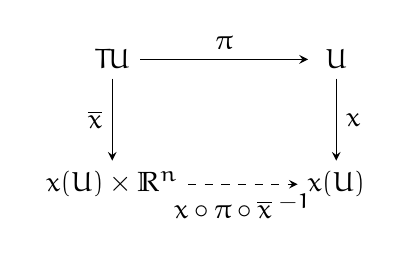
\begin{tikzpicture}
  \matrix (m) [matrix of math nodes,row sep=3em,column sep=4em,minimum width=2em]
  {
     TU & U\\
     x(U) \times \R^n & x(U)\\};
  \path[-stealth]
    (m-1-1) edge node [above] {$\pi$} (m-1-2)
            edge node [left] {$\ol{x}$}  (m-2-1)
    (m-2-1) edge [dashed] node [below] {$x\circ \pi \circ \ol{x}^{\ -1}$} (m-2-2)
    (m-1-2) edge node [right] {$x$} (m-2-2);
\end{tikzpicture}
\end{center}
Como para todo $v \in TU$ el vector $x \circ \pi(v)$ coincide con las primeras $n$ coordenadas de $\ol{x}(v)$, notando $\pi_1 : (p,q) \in \R^n \times \R^n \mapsto p \in \R^n$ es entonces $x\circ \pi \circ \ol{x}^{\ -1} = \pi_1|_{x(U) \times \R^n} \circ \ol{x} \circ \ol{x}^{\ -1}  = \pi_1|_{x(U) \times \R^n}$. Esta \'ultima es diferenciable ya que es la restricci\'on al abierto $x(U) \times \R^n$ de la funci\'on diferenciable $\pi_1$. Consecuentemente, $\pi : TM \to M$ resulta diferenciable.
\end{itemize}
\end{proof}

\begin{obs}{} Sean $M$ una variedad diferenciable y $f \in C^\infty(M)$ una funci\'on que vale constantemente $\mu \in \R$. Si $v : C^\infty(M) \to \R$ es una derivaci\'on en $p \in M$, entonces $v(f) = 0$. En efecto, notando $1 : M \to \R$ a la funci\'on que vale constantemente $1$ es
\begin{align*}
v(1) = v(1 \cdot 1) \stackrel{(Leibniz)}{=} 1(p)v(1) + 1(p)v(1) = 2v(1),
\end{align*}
lo que implica $v(1) = 0$. En consecuencia, $v(f) = v(\mu \cdot 1) = \mu v(1) = 0$.
\end{obs}

Recuerdo ahora el siguiente resultado que utilizar\'e a continuaci\'on,

\begin{proposition}{} Sea $X$ un espacio topol\'ogico conexo y  $f : X \to Y$ una funci\'on. Si $f$ es localmente constante, entonces es constante.
\end{proposition}
\begin{proof} Si $y \in \im f$, el conjunto $E_y := f^{-1}(y) = \{x \in X : f(x) = y\}$ es abierto: para cada $z \in E_y$ existe por hip\'otesis un abierto $U \ni z$ donde $f$ es constante, y como $f(z) = y$ luego $f$ vale constantemente $y$ en todo $U$. Por lo tanto, $z \in U \subset E_y$. Adem\'as los conjuntos $(E_y)_{y \in \im f}$ son disjuntos, pues si $z \in E_y \cap E_{y'}$ entonces $y = f(z) = y'$. Como $X$ es conexo y
\begin{align*}
X = \bigsqcup_{y \in \im f}E_y
\end{align*}
es una uni\'on de abiertos disjuntos no vac\'ios, necesariamente $\#\im f = 1$. Esto es precisamente que $f$ sea una funci\'on constante. 
\end{proof}

\begin{exercise}{12} Sean $M$ y $N$ variedades diferenciables y sea $f:M\to N$ una funci\'on diferenciable. Probar que
\begin{itemize}
\item Si $f$ es constante, entonces $f_{\ast p}=0$ para todo $p\in M$.

\item Si $M$ es conexa y $f_{\ast p}=0$ para todo $p\in M,$ entonces $f$ es
constante.
\end{itemize}
\end{exercise}

\begin{proof} Notaremos $c_q : M \to N$ a la funci\'on que vale constantemente $q$ y definimos $m := \dim M, n := \dim N$. Supongamos en primer lugar que $f = c_q$ para cierto $q \in N$. Sea $p \in M$ y veamos que $f_{\ast p}$ es nula. Dada una derivaci\'on $v : C^\infty(M) \to \R$ en $p$ y $g \in C^\infty(M)$, luego es
\begin{align*}
f_{\ast p}(v)(g) =  v(- \circ f)(g) = v(gf) = v(gc_q) = v(c_{g(q)}) = 0,
\end{align*}
pues notamos anteriormente que las funciones constantes tienen imagen nula por una derivaci\'on. Como $f_{\ast p}(v)$ se anula en toda funci\'on, es $f_{\ast p}(v) = 0$. Por lo tanto, $f_{\ast p}$ se anula en toda derivaci\'on: esto dice que $f_{\ast p} = 0$. Como $p$ era arbitario, $f_{\ast p}$ resulta nula para cualquier $p \in M$.

Supongamos ahora que $M$ es conexa y veamos para este caso la afirmaci\'on rec\'iproca. Alcanza con probar que $f$ es localmente constante: fijemos entonces $p \in M$ y veamos que existe un entorno abierto de $p$ donde $f$ es constante. Consideramos ahora una carta $(V,\psi)$ de $N$ con $f(p) \in V$ y una carta $(U,\varphi)$ de $M$ con $p \in U \subset f^{-1}(V)$ y $U$ conexo\footnote{Como $f$ es continua $f^{-1}(V)$ es abierto, y entonces $f^{-1}(V) \cap U$ es un abierto de $M$ que contiene a $p$. Por lo tanto $f^{-1}(V) \cap U$ es un abierto en $U$, y como \'este es homeomorfo a un abierto eucl\'ideo, tambi\'en lo es $f^{-1}(V) \cap U$. En particular tenemos un entorno conexo $\tilde{U}$ de $p$ contenido en $f^{-1}(V) \cap U$. La restricci\'on de la carta a $\tilde{U}$ es una carta que cumple lo que pedimos, por lo que podemos sin p\'erdida de generalidad asumir directamente a $U$ conexo con $U \subset f^{-1}(V)$.}. Luego, los \textit{ganchos} $\bigg\{\hook{i}{q}{\varphi}\bigg\}_{i=1}^n$ son una base de $T_qM$ para cada $q \in U$. Por hip\'otesis, si $g \in C^\infty(N)$ y $v$ es una derivaci\'on en $q$, es $v(gf) = f_{\ast q}(v)(g) = 0$. En particular,
\begin{align*}
\hook{i}{q}{\varphi}(gf) = \frac{\partial gf\varphi^{-1}}{\partial x_i}\bigg\rvert_{\varphi^{-1}(q)} = 0
\end{align*}
para todo $i \in \nat{m}$ y $q \in U$. Es decir, la funci\'on diferenciable $gf\varphi^{-1} : \varphi^{-1}(U) \to \R$ tiene gradiente nulo. Como $U$ es conexo y $\varphi$ es homeomorfismo, luego $\varphi^{-1}(U)$ es conexo. Como $gf\varphi^{-1}$ tiene gradiente nulo y dominio conexo, es constante:
\begin{align*}
gf\varphi^{-1}(x) = \mu_{g} \in \R \quad (\forall x \in \varphi^{-1}(U)).
\end{align*}
Equivalentemente, se tiene que $gf \equiv c_{\varphi(\mu_g)}$ en $U$ para cada $g \in C^\infty(N)$. Ahora, dado $i \in \nat{n}$ siempre existe $\ol{\psi}^i \in C^\infty(N)$ tal que $\ol{\psi}^i|_V = \psi^i$ y existen entonces constantes $c_1, \dots, c_n \in \R$ tales que $\ol{\psi}^if \equiv c_i$ en $U$. Como $f(U) \subset V$, es
\begin{align*}
c_i \equiv \ol{\psi}^i|_V \circ f\Big|_U^V = \psi^i \circ f\Big|_U^V
\end{align*}
en $U$ para cada $i \in \nat{n}$, de forma que $\psi f \big|_U^V \equiv (c_1, \dots, c_n) =: c$. Como $\psi$ es homeomorfismo, luego $f \big|_U^V \equiv \psi^{-1}(c)$. Vemos as\'i que $f$ es constante en el abierto $U \ni p$, lo que completa la demostraci\'on.
\end{proof}

\end{document}
